% ---- pg-309 （书页 297） ----

\phantomsection\label{eq:7-18}
\begin{equation}
\hat{\epsilon}_j^*=\frac{\hat{\epsilon}_j}{\sqrt{s^2(1-h_{jj})}},\qquad j=1,2,\cdots,n \tag{7-18}
\end{equation}
我们预期学生化残差会大致看上去像是从 $N(0,1)$ 中抽取的独立样本. 某些统计软件包更进一步, 在定义学生化残差时使用``删除一个''方差估计值来估计 $\sigma^2$. 也就是说, 利用将第 $j$ 个观测值从分析中剔除后得出的残差均方 $s_{(j)}$ 来估计 $\sigma^2$.

为了发现可能存在的异常现象, 应将残差用各种方式作图. 对一般的诊断目的来说, 下面各种图形是有用的.

\begin{mvfigure}
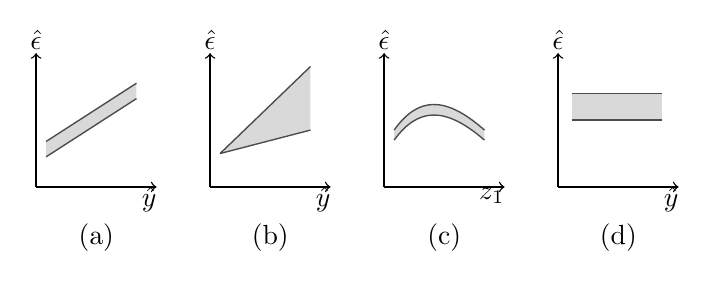
\begin{tikzpicture}[scale=0.85,line width=0.5pt]
% ---- (a) ----
\begin{scope}
\draw[->] (0,0)--(0,2.0);
\node[above,inner sep=1pt] at (0,2.0) {$\hat{\epsilon}$};
\draw[->] (0,0)--(1.8,0);
\node[below left,inner sep=1pt] at (1.85,0.05) {$\hat{y}$};
\fill[black!15] (0.15,0.45)--(1.5,1.32)--(1.5,1.55)--(0.15,0.68)--cycle;
\draw[black!70] (0.15,0.45)--(1.5,1.32);
\draw[black!70] (0.15,0.68)--(1.5,1.55);
\node at (0.9,-0.75) {(a)};
\end{scope}
% ---- (b) ----
\begin{scope}[xshift=2.6cm]
\draw[->] (0,0)--(0,2.0);
\node[above,inner sep=1pt] at (0,2.0) {$\hat{\epsilon}$};
\draw[->] (0,0)--(1.8,0);
\node[below left,inner sep=1pt] at (1.85,0.05) {$\hat{y}$};
\fill[black!15] (0.15,0.5)--(1.5,1.8)--(1.5,0.85)--cycle;
\draw[black!70] (0.15,0.5)--(1.5,1.8);
\draw[black!70] (0.15,0.5)--(1.5,0.85);
\node at (0.9,-0.75) {(b)};
\end{scope}
% ---- (c) ----
\begin{scope}[xshift=5.2cm]
\draw[->] (0,0)--(0,2.0);
\node[above,inner sep=1pt] at (0,2.0) {$\hat{\epsilon}$};
\draw[->] (0,0)--(1.8,0);
\node[below left,inner sep=1pt] at (1.85,0.05) {$z_1$};
\fill[black!15] (0.15,0.7) .. controls (0.5,1.18) and (0.9,1.22) .. (1.5,0.7)
  -- (1.5,0.85) .. controls (0.9,1.38) and (0.5,1.34) .. (0.15,0.85) -- cycle;
\draw[black!70] (0.15,0.7) .. controls (0.5,1.18) and (0.9,1.22) .. (1.5,0.7);
\draw[black!70] (0.15,0.85) .. controls (0.5,1.34) and (0.9,1.38) .. (1.5,0.85);
\node at (0.9,-0.75) {(c)};
\end{scope}
% ---- (d) ----
\begin{scope}[xshift=7.8cm]
\draw[->] (0,0)--(0,2.0);
\node[above,inner sep=1pt] at (0,2.0) {$\hat{\epsilon}$};
\draw[->] (0,0)--(1.8,0);
\node[below left,inner sep=1pt] at (1.85,0.05) {$\hat{y}$};
\fill[black!15] (0.2,1.0)--(1.55,1.0)--(1.55,1.4)--(0.2,1.4)--cycle;
\draw[black!70] (0.2,1.0)--(1.55,1.0);
\draw[black!70] (0.2,1.4)--(1.55,1.4);
\node at (0.9,-0.75) {(d)};
\end{scope}
\end{tikzpicture}
\phantomsection\label{fig:7.2}\mvcap{图 7.2\quad 残差图}
\end{mvfigure}

\noindent\textbf{1.}\quad 残差 $\hat{\epsilon}_j$ 对预测值 $\hat{y}_j=\hat{\beta}_0+\hat{\beta}_1z_{j1}+\cdots+\hat{\beta}_rz_{jr}$ 的标绘图. 对模型假定的偏离常表现在以下两种典型现象之中:

(a) 残差对预测值的依赖性. 这可从\hyperref[fig:7.2]{图 7.2}(a) 得到说明. 引起这种现象的原因是数值计算不正确, 或常数项 $\beta_0$ 在模型中被忽略了.

(b) 方差不总是常数. 残差的模式可能是喇叭状, 如\hyperref[fig:7.2]{图 7.2}(b) 所示, 因此 $\hat{y}$ 值增大时变差也增大, $\hat{y}$ 值变小时变差亦变小. 在这种场合, 误差方差不是常数. 这时要求采用适当的变换或采用加权最小二乘法, 也可二者同时采用(见练习 7.3).

在\hyperref[fig:7.2]{图 7.2}(d) 中, 残差形成一条水平带. 这是理想状态, 表明残差的方差相等且不依赖于 $\hat{y}$.

\noindent\textbf{2.}\quad 残差 $\hat{\epsilon}_j$ 对某个预测量(例如 $z_1$)或预测量的乘积(如 $z_1^2$ 或 $z_1z_2$)的标绘图. 这些标绘图中的某种系统变化模式暗示需要在模型中加入更多的项. 这个情况由\hyperref[fig:7.2]{图 7.2}(c) 中说明.

\noindent\textbf{3.}\quad \textbf{$Q$-$Q$ 图和直方图.} 误差是否显示正态分布? 为了回答此问题, 残差 $\hat{\epsilon}_j$ 或 $\hat{\epsilon}_j^*$ 可用 4.6 节中所讨论的方法来检查. $Q$-$Q$ 图、直方图和点图有助于发现非正常数据或对正态性的严重偏离(这在分析中需要特别注意). 若 $n$ 很大, 则对正态性的少许偏离不会对 $\boldsymbol{\beta}$ 的推断产生太大影响.

\noindent\textbf{4.}\quad \textbf{残差对时间的标绘图.} 关于独立性的假定十分重要, 但难于检查. 若数据按自然的时间顺序排列, 则残差对时间的标绘有可能揭示某种系统模式.(残差对空间位置的标绘也可能揭示诸误差之间的联系.) 例如, 残差随时间增大表明存在某种强正相关性. 独立性的统计检验可以通过一阶自相关系数
\phantomsection\label{eq:7-19}
\begin{equation}
r_1=\frac{\sum\limits_{j=2}^{n}\hat{\epsilon}_j\hat{\epsilon}_{j-1}}{\sum\limits_{j=1}^{n}\hat{\epsilon}_j^2} \tag{7-19}
\end{equation}
来构造. 一种常用的检验方法以统计量 $\sum\limits_{j=2}^{n}(\hat{\epsilon}_j-\hat{\epsilon}_{j-1})^2\Big/\sum\limits_{j=1}^{n}\hat{\epsilon}_j^2\doteq 2(1-r_1)$ 为依据, 这种检验称
